\section{Prosedur Penelitian dan Pengembangan}


\subsection{Data Penelitian}
    
Berdasarkan studi kasus dalam skripsi ini, data yang akan digunakan dalam penelitian ini adalah data koordinat dari seluruh SMA di Kabupaten Probolinggo. Data nama-nama sekolah dikumpulkan dari \url{https://data.sekolah-kita.net}, dan data koordinat dikumpulkan melalui aplikasi Google Earth yang dapat diunduh langsug ke dalam bentuk excel. Waktu yang diperlukan peneliti untuk mengumpulkan data dari web tersebut kurang lebih sekitar satu bulan.

\subsection{Instrumen Pendukung}
\begin{enumerate}
    \item Python
    
    Dalam penelitian ini akan digunakan bahasa pemrograman python untuk mempermudah pengerjaan. Bahasa python adalah bahasa pemrograman baru di masa sekarang, karena dalam bahasa ini lebih simple dan singkat dalam membuat program \cite{syahrudin2018input}. Bahasa pemrograman ini merupakan bahasa pemrograman yang paling mudah dipelajari dari pada bahasa pemrograman yang lain. Serta dalam bahasa pemrograman ini dapat menjalankan beberapa rumus matematika di dalamnya. Selain itu bahasa Python telah digunakan secara luas, dan masuk dalam 3 besar bahasa pemrograman yang digunakan dalam beberapa tahun belakangan.
    
    \item Jupyter Notebook
    
    Jupyter Notebook adalah aplikasi web gratis yang digunakan untuk membuat dan membagikan dokumen yang memiliki kode, hasil hitungan, visualisasi, dan teks. Notebook ini juga mendukung 3 bahasa pemrograman salah satunya adalah bahasa pemrograman python. Banyak kelebihan yang disajikan dari aplikasi ini salah satunya adalah visualisasi data, mendokumentasikan kode, dan menjalankan kode dalam setiap sel.

\begin{figure}[h!]
  \centering
  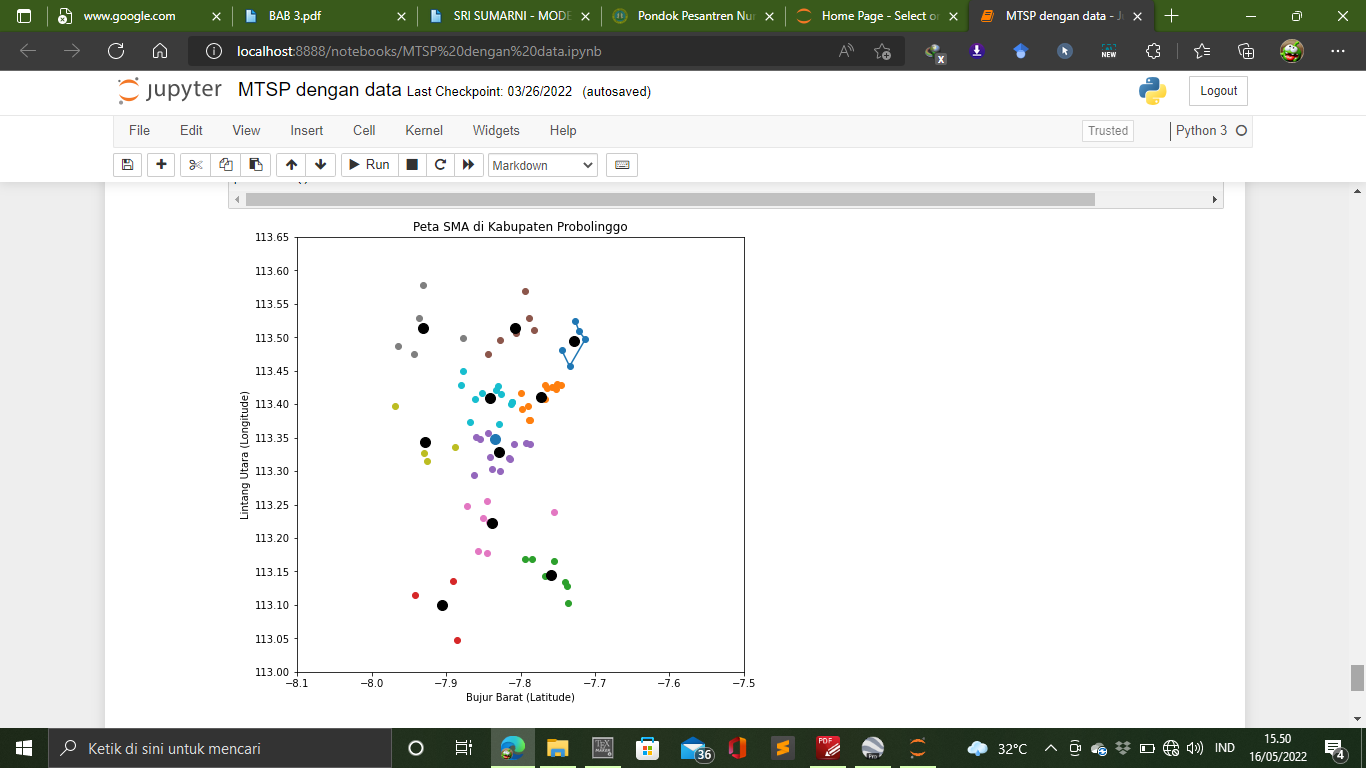
\includegraphics[width=0.8\textwidth]{visualisasi jupyter.png}
  \caption{Visualisasi data menggunakan jupyter notebook}
\end{figure}

	\item Google Earth
	
	Google earth digunakan dalam penelitian ini untuk mengumpulkan koordinat lokasi seluruh SMA di Kabupaten Probolinggo. Dalam hal ini google earth dapat menandai beberapa lokasi dan mengekspor langsung kedalam bentuk excel. Data-data lokasi yang telah didownload ke dalam bentuk excel akan diproses menggunakan jupyter notebook.

\begin{figure}[h!]
  \centering
  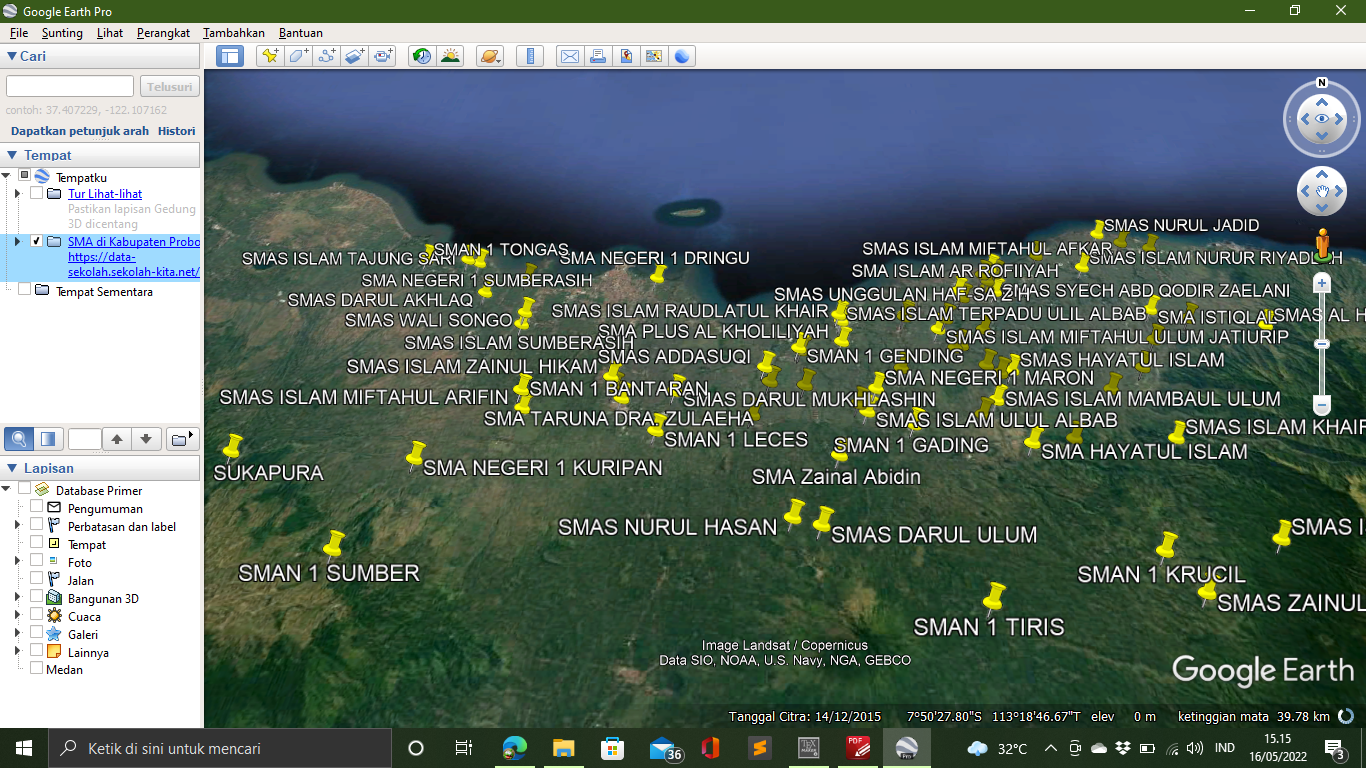
\includegraphics[width=0.8\textwidth]{google earth.png}
  \caption{Menandai beberapa lokasi pada google earth}
\end{figure}

\begin{figure}[h!]
  \centering
  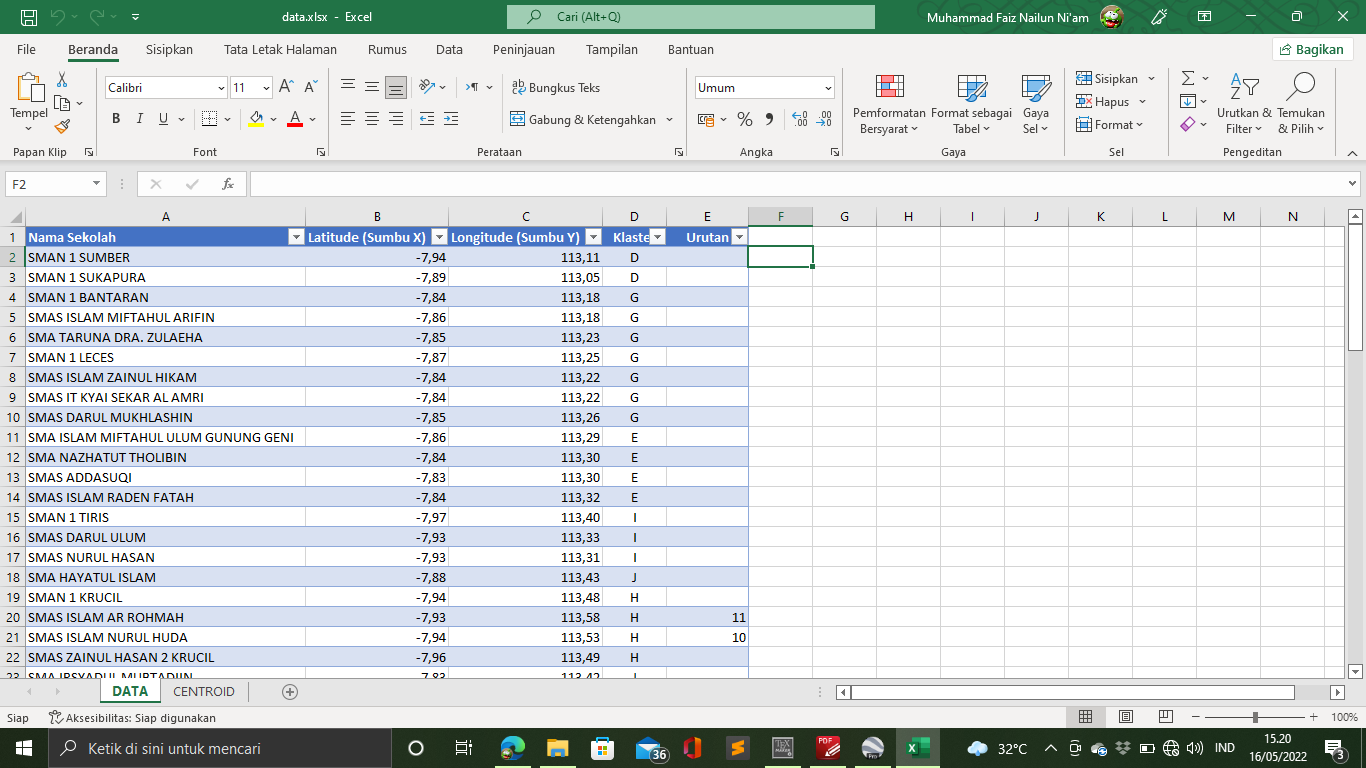
\includegraphics[width=0.8\textwidth]{ekspor excel.png}
  \caption{Mengekspor data dan menjadikannya ke format excel}
\end{figure}

\end{enumerate}

\subsection{Langkah-langkah Dalam Tahap Pengolahan Data}
\begin{enumerate}
    \item Menyiapkan data yang telah dikumpulkan sebelumnya.
    \item Selanjutnya menentukan jumlah klaster yaitu sebanyak $n$ klaster. Data yang telah dikumupulkan pada tahap ini akan dibagi menjadi beberapa klaster, metode yang digunakan algoritma \textit{k}-means.
    \item Langkah-langkah yang digunakan dalam metode \textit{k}-means adalah sebagai berikut
    \begin{enumerate}
        \item Memilih sebanyak $n$ \textit{centroid} secara acak, sesuai dengan berapa banyak salesman yang akan ditugaskan
        \item Menghitung jarak data ke \textit{centroid} dengan rumus \textit{euclidean distance}
        \begin{equation}
        d_{xy}=\sqrt{\sum_{i=1}^{n}(x_i-y_i)^{2}}
        \end{equation}
        \item Titik-titik lokasi yang tersebar merupakan klaster yang sama dengan titik \textit{centroid} paling dekat
        \item Perbarui \textit{centroid} tiap klaster yang dihasilkan dengan menghitung nilai koordinat rata-rata titik nilai pada masing-masing klaster.
        \item Iterasi dilakukan untuk generasi berikutnya sampai yaitu dengan kembali ke tahapan (b) sampai tidak ada perubahan klaster atau perubahan nilai \textit{centroid}
    \end{enumerate}
	
	\item Selanjutnya melakukan proses TSP pada setiap klaster yang telah dibagi, langkah-langkahnya adalah sebagai berikut.
	\begin{enumerate}
	    \item Membuat populasi awal secara random menggunakan data yang telah diklaster
	    \item Melakukan reproduksi dengan metode \textit{crosover} dengan peluang 0,95
	    \item Melakukan mutasi pada data dengan peluang 0,01
	    \item Selanjutnya seleksi dengan mode eliminasi
	    \item Menentukan nilai fitness agar mendapatkan solusi akhir yang optimal dengan rumus:
	    \begin{equation}
	    fitness=\frac{10000}{RMSE}
	    \end{equation}
	    \item Iterasi dilakukan dengan cara kembali ke tahapan b untuk generasi berikutnya sampai hasil yang dilakukan optimal atau mendekati optimal.
    \end{enumerate}
	\item Ketika proses diatas selesai dilakukan maka dihasilkanlah pembagian klaster dan rute terdekat tiap klaster menuju seluruh SMP di Kabupaten Probolinggo
	\item Mengevaluasi data yang dihasilkan
\end{enumerate}